\chapter{Propuesta}\label{chapter:proposal}
 
    El objetivo de desarrollar un sistema para generar resúmenes de eventos deportivos independiente de la fuente de datos 
planteó distintos retos. El primero de estos fue la necesidad de definir un esquema que permitiera abstraer las características 
generales del conjunto de deportes de enfrentamiento (enfrentamiento dos a dos). Junto con dicho esquema se necesitó 
deifinir una estructura común para la entrada de los datos que permitiera expresar los conocimientos del dominio. Se seleccionó 
una estructura basada en tuplas de cuatro elementos (cuatro-tupla en lo adelante). A partir de esta estructura y en base 
al esquema de definición general se buscó poder determinar esquemas específicos para cada deporte que se fuera a incluir en el 
sistema. Cada uno de estos esquemas específicos son los que se encargan de definir un deporte de forma individual dentro del sistema.
    
    La segunda parte del trabajo consistió en construir en base a la propuesta, un esquema y su modelo correspondiente para generar 
resúmenes de partidos de fútbol. Lo mismo se realizó con un deporte de naturaleza diferente como el boxeo.

\section{Propuesta de Esquema General}

    Los deportes se pueden clasificar en la categoría de individuales o colectivos. En los deportes colectivos, las representaciones 
del enfrentamiento ocurren en base a equipos que agrupan a individuos. A su vez en los deportes individuales son dos los contendientes.
Esta es la primera diferencia que se extrae en el análisis del conjunto de deportes. Las modalidades analizadas entán representadas en \ref{tab:table_deportes_seleccionados}, 
clasificadas en individuales o colectivas.

% Please add the following required packages to your document preamble:
% \usepackage{multirow}
\begin{table}[]
    \begin{center}
    \begin{tabular}{|c|c|}
    \hline
    Colectivos                                                                                                                                          & Individuales                                                                                                     \\ \hline
    \multirow{5}{*}{\begin{tabular}[c]{@{}c@{}}Béisbol, Voleibol, \\ Fútbol, Tenis Dobles, \\ Baloncesto, Waterpolo, \\ Balonmano, Hockey\end{tabular}} & \multirow{5}{*}{\begin{tabular}[c]{@{}c@{}}Tenis, Esgrima, \\ Boxeo, Judo,\\ Lucha libre, Taekwondo\end{tabular}} \\
                                                                                                                                                        &                                                                                                                  \\
                                                                                                                                                        &                                                                                                                  \\
                                                                                                                                                        &                                                                                                                  \\
                                                                                                                                                        &                                                                                                                  \\ \hline
    \end{tabular}
    \caption{Deportes analizados}
    \label{tab:table_deportes_seleccionados}
    \end{center}
\end{table}

    De cada uno de estos deportes se analizó:

    \begin{itemize}
        \item Naturaleza de decisión: La mayoría de los deportes se definen como juegos 
        adversariales por acumulación de puntos. La entidad con mayor puntuación gana. Otros como el tenis y el voleibol 
        se definen por cantidad de etapas ganadas (sets), y cada etapa se gana por puntos. A su vez en el boxeo la definición 
        se deriva de votaciones de árbitros.
        \item Posibilidad de empate: Hay deportes como el fútbol que según la competición existe la posibilidad de 
        definirse sin ganadores ni perdedores
        \item Division de los eventos: La mayoría de los eventos se divide por etapas de tiempo
        constante. Una excepción es el judo que ocurre de forma continua durante cuatro minutos. 
        \item Alargues de tiempo: La mayoría de los deportes, en caso de no definición en su tiempo reglamentario presentan 
        etapas adicionales en forma punto de oro (ej. judo),  tiempos extras (ej. béisbol, fútbol), tiebreak (desemapte, ej. Voleibol, tenis).
        \item Roles: Dentro de los deportes los participantes ejercen roles, como puede ser su posición en los deportes colectivos. En los deportes 
        individuales estos roles no son tan explícitos.
        \item  Acciones principales: La definición de los eventos son las acciones relevantes que ocurren durante el tiempo de juego.
    \end{itemize}

    Del análisis también se extrajeron un conjunto de características que son comunes a los enferntamientos deportivos: la sede, 
el público, la fecha. Así mismo, los enfrentamientos normalmente se encuadran dentro de un torneo, y existen distintiones entre categorías lo mismo sea 
de edad, sexo, u de otro tipo (ej. peso).

    A partir del análisis se definió un meta esquema general de tipos de entradas basado en una estructura de 
cuatro-tuplas de conocimiento.

\begin{table}[]
    \begin{center}

\begin{tabular}{|c|c|}
    \hline
    Tipo de Entrada  & Estructura                                                                                                               \\ \hline
    SEDE             & \begin{tabular}[c]{@{}c@{}}(TipoSEDE, \\ Nombre\\ Asistencia\\ Capacidad)\end{tabular}                                   \\ \hline
    TORNEO           & \begin{tabular}[c]{@{}c@{}}(TipoTORNEO\\  Nombre\\ Expresión de Género\\  Expresión de Categoría)\end{tabular}           \\ \hline
    ENFRENTAMIENTO   & \begin{tabular}[c]{@{}c@{}}(TipoENFRENTAMIENTO\\ Entidad\_1\\  Entidad\_2\\  Expresión de Fecha)\end{tabular}            \\ \hline
    ROLENJUEGO       & \begin{tabular}[c]{@{}c@{}}(TipoROLENJUEGO\\  Entidad del Rol\\  Entidad Complementaria\\ Rol Complementario)\end{tabular}   \\ \hline
    RESULTADOPARCIAL & \begin{tabular}[c]{@{}c@{}}(TipoRESULTADOPARCIAL\\ Entidad\\ Indicador de parcial\\ Expresión de puntuación)\end{tabular}    \\ \hline
    RESULTADOFINAL   & \begin{tabular}[c]{@{}c@{}}(TipoRESULTADOFINAL\\ Entidad\\ Expresión de puntuación\\  Descriptor de resultado)\end{tabular}  \\ \hline
    EVENTO           & \begin{tabular}[c]{@{}c@{}}(TipoEVENTO\\  Expresión de Tiempo\\ Entidad Protagonista\\  Entidad Complementaria)\end{tabular} \\ \hline
    \end{tabular}
        
    \end{center}
    \caption{Meta esquema general para definir las entradas de cada deporte}
    \label{tab:esquema_general}
\end{table}

    Cada cuatro-tupla tiene en la primera posición el tipo de entrada. El resto de los valores constituyen la base de información. Con cada tipo de entrada 
se encapsula un subconjunto de la información que se muestra, común al conjunto de deportes estudiados. 
    A patir del meta esquema general, es posible definir los esquemas específicos de cada deporte, con sus tipos particulares para cada entrada y su forma de interpretar 
cada uno de los valores. Los esquemas de cada deporte tienen que ser capaces de poder expresar la información del mismo para poder, a través de ella, 
generar textos que describan el evento. A continuación se presenta la definición para dos deportes de naturaleza y estructura muy dispar: el fútbol y 
el boxeo.


\section{Definición y modelo generador para el fútbol}

    Es necesario antes de la introducción del modelo la definición del esquema específico que se utilizó para 
definir y validar las posibles entradas del sistema.

\subsection{Esquema de entrada de datos}

    La experiencia del autor sobre el dominio a tratar así como la consulta del sitio web \textit{whoscored.com} sirvieron para realizar la caracterización del 
fútbol como deporte. Trabajos previos que también abordaron este deporte para la generación de texto como (~\cite{theune2001data,aires2016automatic,van2017pass}) se tuvieron en cuenta. 
El sitio \textit{whoscored.com} publica estadísticas y anotaciones de los eventos que ocurren durante un partido de fútbol y dispone de información de miles de encuentros.

A partir de este análisis, se definió el esquema del fútbol como se muestra en \ref{tab:esquema_futbol}

\begin{table}[]
    \begin{center}
        

\begin{tabular}{|c|c|}
    \hline
    Tipo de Entrada  & Valores en el Esquema del Fútbol                                           \\ \hline
    SEDE             & Estadio                                                                    \\ \hline
    TORNEO           & Torneo                                                                     \\ \hline
    ENFRENTAMIENTO   & PartidoPresentacion                                                        \\ \hline
    ROLENJUEGO       & \begin{tabular}[c]{@{}c@{}}Titular\\ Suplente\end{tabular}                 \\ \hline
    RESULTADOPARCIAL & \begin{tabular}[c]{@{}c@{}}Tiempos\\ TiemposExtras\\ Penaltis\end{tabular} \\ \hline
    RESULTADOFINAL   & ResultadoFinal                                                             \\ \hline
    EVENTO &
      \begin{tabular}[c]{@{}c@{}}PaseBueno,PaseFallado,PaseClave,PaseAsistencia,\\ TiroPuerta,TiroNoPuerta,Gol,Atajada,\\ EntradaConExito,EntradaFallada,BloqueoDeDisaparo,\\ Recuperación,FaltaFueraDelArea,ManoFueraDelArea,\\ FaltaDentroDelArea,ManoDentroDelArea,PenaltiCometido,\\ AtajadaPenalti,GolPenalti,TiroPenaltiFuera,TarjetaAmarilla,\\ SegundaTarjetaAmarillaRoja,TarjetaRojaDirecta,\\ GolTiroLibre,Autogol,CobraCorner,Cambio,FueraDeJuego\end{tabular} \\ \hline
    \end{tabular}
    \end{center}   
    \caption{Esquema de definición del fútbol}
    \label{tab:esquema_futbol}
\end{table}

Cada esquema presenta sus especificaciones en cuanto a la intrepretación o la representación de los 
valores por tipo de entrada. Este esquema establece las siguientes:

    \begin{itemize}
        \item Tupla \textbf{SEDE}: Las expresiones de \textit{asistencia} y \textit{capacidad} de no ser vacías deben ser expresiones numéricas (ej. “1200”).
        \item Tupla \textbf{TORNEO}: La expresión de \textit{género} debe ser una entre “M” y “F” (masculino, femenino). 
        \item Tupla \textbf{ENFRENTAMIENTO}: Las entidades son los nombres de los equipos que se enfrentan. La expresión de \textit{fecha}, de ser incluida, debe seguir
        el siguiente formato: “AAAA-MM-DD HH:MM” (año-mes-día hora:minutos). Es posible que se provea solo el día o la hora, respetando sus formatos específicos.
        \item Tupla \textbf{ROLENJUEGO}: La entidad de Rol es el jugador, y la entidad complementaria su equipo. El \textit{Rol Complementario} indica la posición que 
        desempeña el jugador en el terreno. Debe ser uno entre: \textit{“POR”} (portero), \textit{“DEF”} (defensa), \textit{“CEN”} (centrocampista) o \textit{“DEL”} (delantero).
        \item Tupla \textbf{RESULTADOPARCIAL}: La entidad es el equipo al que se refiere, el \textit{indicador de parcial} un valor entre 1 y 5 que se refiere al número de la etapa. Para  
        los \textit{Tiempos} los valores son 1 y 2, para los \textit{TiemposExtra}, 3 y 4, y para \textit{Penaltis}, el 5.
        \item Tupla \textbf{RESULTADOFINAL}: La entidad es el equipo al que se refiere, la \textit{puntuación} es la cantidad de goles anotados por el equipo. El \textit{descriptor de 
        resultado} es uno entre “V” (victoria), “E” (empate) , “D” (derrota).
        \item Tupla \textbf{EVENTO}: La \textit{expresión temporal} tiene el siguiente formato: “p\_MM\_SS”, donde p es un indicador del segmento de juego en el que ocurrre la acción. 
        La entidad \textit{protagonista} es el jugador que, valga la redundancia, protagoniza el evento, mientras que el \textit{complementario} es el jugador que complementa la 
        información del evento y se requiere principalmente en acciones como el “Cambio”, respondiendo a ¿de quién?, ¿por quién?.
    \end{itemize}

    Como se busca que el sistema pueda ser adaptable por el usuario a distintas fuentes de datos, no es obligatorio proveer todo el conjunto de información para 
obtener un resultado. En cambio, si existe un conjunto minimal de información que el sistema requiere, como el resultado y el torneo y la estructura de los equipos. 
Una formación inadecuada de las tuplas de los eventos conllevará a incongruencias del texto producido respecto al partido en cuestión, pero no es objetivo de 
este trabajo evaluar la factibilidad de la obtención de los datos o su adaptabilidad a la estructura planteada.


\subsection{Generación del reporte}

    Con el objetivo de generar rerportes resumidos de partidos de fútbol a patir de las tuplas de conocimiento de los partidos, el sistema propuesto adapta enfoques presentados 
en la literatura para esta problemática en idiomas distintos al español. La arquitectura general planteada se presenta en \ref{arquitecturadelmodelo} y constituye una 
adaptación de la propuesta en (~\cite{aires2016automatic}) que a su vez sigue un enfoque basado en (~\cite{theune2001data}). A diferencia de ambas propuestas, el 
presente sistema no consume bases de conocimiento del dominio específico a abordar ya que no se enfoca únicamente en una competición, sino que busca adaptarse al hecho 
general de un partido de fútbol. 
%Estos, lo mismo pueden pertenecer a eventos tipo Liga, donde los partidos duran 90 minutos y existen empates, o a eventos de eliminación 
%directa donde los partidos deben tener una definición ya sea en tiempos extras o penales.


\begin{figure}[!]
    \begin{center}
        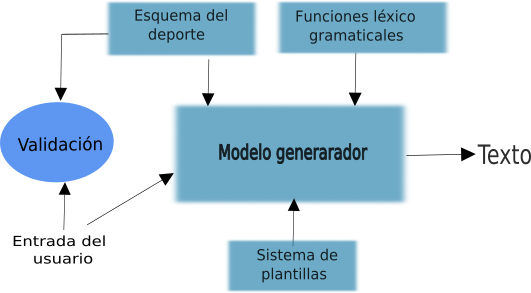
\includegraphics[scale=0.9]{Graphics/arquitecturaprop2.png}
    \end{center}
    \caption{Arquitectura del modelo propuesto}
    \label{arquitecturadelmodelo}
\end{figure}

    El módulo de generación hace uso de plantillas de expresiones creadas a mano. Con las plantillas se busca la 
construcción de oaciones que expresen distintos eventos relevantes que ocurren dentro del partido. Para la selección de 
los eventos y la determinación de las piezas importantes dentro de la estructura se analizó un conjunto de crónicas de partidos. 
Se busca que el texto producido tenga cierto grado de variabilidad y que sea correcto en cuanto a estructura y gramática.


\subsection{Planificación de contenido}

    En orden de estructurar el texto a producir así como determinar los eventos relevantes de un partido se hizo un análisis basado en 
corpus (~\cite{reiter_dale_2000}). Se seleccinaron 4 jornadas (las 22,23,24,25) de la Liga Española de Fútbol Profesional de la temporada 
2021-2022. Así mismo se seleccinó dos medios de prensa que realizaron crónicas en español de estos partidos en su versión web. Estos medios 
fueron: el \textit{Diario AS\footnote[1]{https://as.com/}} en su versión web \textit{As.com} y el sitio deportivo 
\textit{ESPN Deportes\footnote[2]{https://espndeportes.espn.com/}}. Para determinar que eventos eran narrados en cada crónica se 
estudiaron los eventos ocurridos en cada partido anotados por una tercera fuente, el sitio estadístico \textit{www.whoscored.com}. 
De los 40 juegos se hizo una selección de 15 que tuvieran presente la información en ambos medios para poder constrastar. Los resultados de las 
menciones de cada evento se pueden obeservar en la tabla (\ref{tabla-eventos}).\\



            INSERTAR TABLA EVENTOS.\\

    Se determinan tres piezas comunicativas: las presentación del resultado, la descripción de los eventos relevantes y 
la mención de jugadores con una destacada actuación. En base a esto se definió la siguiente estructura:

\begin{itemize}
    \item Presentación del partido: Una primera oración donde se presentan los equipos y el resultado final del encuentro.
    \item Mención de los eventos relevantes: Se van contando los eventos relevantes del partido en orden cronol\'ogico.
    \item Jugador más destacado: Se hace una mención del jugador más destacado del encuentro en base a las estadísticas extraídas de los 
    eventos. En caso de no existir una actuación destacada se expresa este hecho.
\end{itemize}


    \textbf{Presentación}\\

    Los juegos de fútbol presentan variedad en cuanto a sus momentos de decisión. Estos, lo mismo pueden pertenecer a eventos tipo Liga, donde los partidos 
duran 90 minutos y existen empates, o a eventos de eliminación directa donde los juegos deben tener una definición ya sea en tiempos extras 
o en tandas de penales (\ref{fig_momentos_definicion}). Para cada uno de estos tipos de 
definición se definen plantillas específicas a la hora de construir la presentación. Así mismo, en la presentación se incluye la información 
respectiva a la sede donde se desarrolla el encuentro.\\

    \begin{figure}[!]
        \begin{center}
            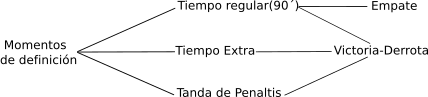
\includegraphics[scale=1]{Graphics/momentodef.png}
        \end{center}
        \caption{Momentos de definición de un partido de fútbol}
        \label{fig_momentos_definicion}
    \end{figure}

    \textbf{Eventos relevantes}\\

    Se determinó como eventos relevantes a incluir en el resumen aquellos que tienen una influencia directa 
tanto en el resultado como en el transcurso del juego. Por tanto los eventos seleccionados son: los goles y asistencias, 
las expulsiones y los fallos de penaltis. Cada uno de ellos se presenta en oraciones independientes y poseen plantillas de acuerdo 
a su clasificación. En \ref{fig_clasificacioneventos} se muestran las distintas clasificaciones de los eventos relevantes.\\


    \begin{figure}[!]
        \begin{center}
            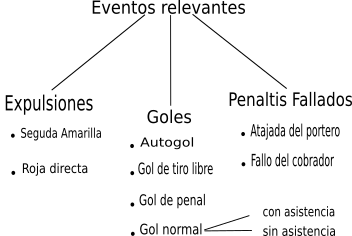
\includegraphics[scale=0.9]{Graphics/clasificacioneventosrel.png}
        \end{center}
        \caption{Clasificación de los eventos relevantes}
        \label{fig_clasificacioneventos}
    \end{figure}

    \textbf{Jugador destacado}\\

    El conjunto de acciones que se pueden describir del juego (ver eventos en \ref{tab:esquema_futbol}) se utilizaron para 
determinar el jugador más destacado del partido. Se planteó una heurística en base a asignar distinta aportación de valor a 
las acciones. Así mismo, acciones negativas se penalizan con evaluaciones negativas. En \ref{tab:tablaheuristica} se muestan los valores utilizados.



\begin{table}[]
    \begin{center}
        

    \begin{tabular}{|c|c|llcc}
    \cline{1-2} \cline{5-6}
    \textbf{Estadística} &
      \textbf{Valor aportado} &
      \multicolumn{2}{l|}{\multirow{4}{*}{}} &
      \multicolumn{1}{c|}{\textbf{Estadística}} &
      \multicolumn{1}{c|}{\textbf{Valor aportado}} \\ \cline{1-2} \cline{5-6} 
    Goles            & x3    & \multicolumn{2}{l|}{}    & \multicolumn{1}{c|}{Recuperaciones} & \multicolumn{1}{c|}{x0.2}    \\ \cline{1-2} \cline{5-6} 
    Autogoles        & x(-3) & \multicolumn{2}{l|}{}    & \multicolumn{1}{c|}{Pases buenos}   & \multicolumn{1}{c|}{x0.02}   \\ \cline{1-2} \cline{5-6} 
    Asistencias      & x1.5  & \multicolumn{2}{l|}{}    & \multicolumn{1}{c|}{Pases malos}    & \multicolumn{1}{c|}{x(-0.1)} \\ \cline{1-2} \cline{5-6} 
    Atajadas         & x1    &  & \multicolumn{1}{l|}{} & \multicolumn{1}{c|}{Tiros a puerta} & \multicolumn{1}{c|}{x0.2}    \\ \cline{1-2} \cline{5-6} 
    Penales atajados & x2    &  & \multicolumn{1}{l|}{} & \multicolumn{1}{c|}{Tajeta Roja}    & \multicolumn{1}{c|}{x(-2)}   \\ \cline{1-2} \cline{5-6} 
    Pases claves     & x0.25 &  & \multicolumn{1}{l|}{} & \multicolumn{1}{c|}{Tareta amrilla} & \multicolumn{1}{c|}{x(-0.5)} \\ \cline{1-2} \cline{5-6} 
    Entradas buenas  & 0.1   &  &                       &                                     &                              \\ \cline{1-2}
    \end{tabular}
    \end{center}
    \caption{Valores que aporta cada estadística}
    \label{tab:tablaheuristica}
    \end{table}

    En busca de representar en cierta medida el valor subjetivo que tiene el gol como acción principal de un partido de fútbol se agrega valor a los jugadores que 
consigue más de una anotación. Si un jugador anota dos goles se le suma medio punto, si anota tres, 1, y si consigue más de tres goles se le adicionan 3 puntos. 
Si un jugador anota el gol de la victoria de su equipo, se le 
adiciona un punto.  Se considera gol de la victoria al último gol del partido si la diferencia final entre los dos equipos es de un solo gol. A los 
jugadores de corte defensivo (portero y defensas) también se les agrega un punto si su equipo no recibe goles. Los jugadores del equipo que resulta derrotado ven 
reducido sus puntos en un diez por ciento. El jugador con mayor puntuación del partido se considera el hombre del partido.



\subsection{Realización}

    En la etapa de realización del texto, vemos unificadas las tareas de carácter lingüístico tal y como se presentó en \ref{chapter:state-of-the-art}. 
En este proceso se definen las palabras y expresiones con las que expresar el contenido seleccionado bajo la estructura definida. El enfoque basado en reglas 
y llenado de plantilla es de los más utilizados por el control que otorga sobre la producción del texto (\ref{subsection:lexicalizacion}). Tiene la ventaja de que 
se asegura la calidad estructural del texto producido, así como permite dotar de variabilidad a las salidas tal y como se discutió en \ref{subsection:realizcion}.

    Las plantillas pueden o no presentar ranuras para completar con información. Las ranuras se utilizan de la forma: \textit{$<$ dato $>$} donde 
\textit{dato} se sustituye por el valor de la variable que representa. Para dotar de facilidad al sistema a la hora de adaptarse a eventos de 
ambos géneros se utilizan dentro de las plantillas expresiones como \textit{\$ palabra \$}, donde \textit{palabra} se sustituye por su expresión de 
género correcta dentro del contexto a través de una de las funciones léxicas que se utilizan en el modelo. 

    Cuando una oración queda estructurada en base a las expresiones que la conforman y los valores de las ranuras se rellenan con los datos reales, entonces 
se utiliza una función para dar formato a la oración. En dicha función se colocan las mayúsculas al comienzo de la oración así como el punto final. También se 
elimninan los espacios en blanco que pudieran quedar de más por datos faltantes, y se corrigen situaciones como la repetición de artículos o de palabras.
    Las plantillas se utilizan dentro del modelo para conformar estructuras más complejas en forma de 
oraciones. Cada conjunto de plantillas dentro del sistema pertenece a una parte de la estructura del texto definida en el ep\'igrafe anterior y como 
tal se analizará a continuación.\\

    \textbf{Presentación}\\

    En el texto de presentación se busca expresar la información concerniente al resultado del partido, su cirscunstancia, así como el lugar donde se 
realiza este. Se plantea en forma de oración que sigue una de estas estructuras de forma aleatoria:
    \begin{itemize}
        \item \textit{plantilla de estadio} $+$ ", " $+$ \textit{plantilla de resultado}
        \item \textit{plantilla de resultado} + \textit{plantilla de estadio}
    \end{itemize}
        
Las \textit{plantilla de estadio} se escogen en relación a si se conoce o no el valor de la asistencia al partido, pudiendo tener las siguiente expresiones:
    \begin{itemize}
        \item \textit{con  $<$ asistencia $>$ hinchas en las gradas del estadio $<$ estadio $>$}
        \item \textit{en el estadio $<$ estadio $>$}
    \end{itemize}

Las \textit{plantilla de resultado} se construyeron en distintos grupos en dependencia del resultado del partido y el momento de definición:
    \begin{itemize}
        \item Se define en tiempo regular: Estos pueden ser empate o con ganador. 
                    \begin{itemize}
                        \item Si el resultado es empate, se tienen los subgrupos: empate con goles, 
                        empate con uno o dos goles, empate con más de dos goles. 
                        \item  Si hay un ganador definido, se tiene dos subgrupos: resultado normal, 
                        resultado por goleada. Se toma como resultado por goleada cuando la diferencia es de tres o más goles
                    \end{itemize}
        \item Se define en tiempo extra
        \item Se define en tanda de penaltis.
    \end{itemize}

    Ejemplos de construcción:

        \begin{itemize}
           \item  \textit{ con  $<$ asistencia $>$ hinchas en las gradas del estadio $<$ estadio $>$, en tiempo extra $<$ equipo\_ganador $>$ superó $<$ equipo\_ganador\_goles $>$ a \\$<$ equipo\_perdedor\_goles $>$ a $<$ equipo\_perdedor $>$ }
        
            \item  \textit{$<$ equipo\_ganador $>$ goleó a $<$ equipo\_perdedor $>$ $<$ equipo\_ganador\_goles $>$ \\a $<$ equipo\_perdedor\_goles $>$ en el estadio $<$ estadio $>$}
        \end{itemize}



\textbf{Eventos principales}\\


    Las expulsiones se expresan a través de un de las siguientes estructuras:
    \begin{itemize}
        \item \textit{plantilla tiempo} + \textit{plantilla tipo expulsión}
        \item \textit{plantilla tipo expulsión} + \textit{plantilla tiempo}
    \end{itemize}

    Las \textit{plantillas de tiempo} son del tipo: \textit{cuando corría el minuto $<$ minuto $>$}

    Los penaltis fallados siguen una estructura similar:
    \begin{itemize}
        \item \textit{plantilla tiempo} + \textit{plantilla tipo fallo}
        \item \textit{plantilla tipo fallo} + \textit{plantilla tiempo}
    \end{itemize}

    Ejemplos de construcciones: 

    \begin{itemize}
    \item Expulsión por segunda amarillas:  \textit{una segunda amarilla a $<$ jugador\_expulsado $>$ dejó 
    a $<$ equipo\_jugador\_expulsado $>$ con $<$ jugadores\_restantes $>$ sobre el terreno 
    en el minuto $<$ minuto $>$}
    
    \item Penalti atajado: \textit{en el $<$ minuto $>$, $<$ lanzador $>$ tuvo la oportunidad 
    para $<$ equipo\_lanzador $>$ desde el punto de penal pero $<$ portero $>$ le detuvo el lanzamiento}
    \end{itemize}


    Para la expresión de los goles se utilizan las plantillas: \textit{tipo de gol}, \textit{resultado del gol}, 
    \textit{asistencia}, \textit{tiempo}. Para los goles se identifican cuatro tipos: autogol, gol de tiro libre, 
    gol de penal y gol simple. A su vez, las cirscunstancias del partido condicionan a la hora de expresar el resultado 
    de un gol. Se identifica que un gol puede ser el primer gol del partido, o el único gol del partido, o puede empatar 
    un resutado, desemaptar un resultado, aumentar la ventaja o disminuir la ventaja.
    Se escoge entre 14 estructuras de oraciones de forma aleatoria a la hora de realizar una acción de gol. Se presentan tres 
    de estas estructuras, las restantes son variaciones estructurales de las mismas.
    
    %“ ” 

    \begin{itemize}
        \item \textit{ “con ” + plantilla\_tipo\_gol + “ ” + plantilla\_asistencia+ “, ”+ autor\_del\_gol + “ ” + plantilla\_resultado\_de\_gol + “ ” + plantilla\_tiempo}
        \item \textit{plantilla\_tiempo + “, ” + plantilla\_tipo\_gol + “ de ”+ autor\_del\_gol + “, ” + plantilla\_asistencia + “, ” + plantilla\_resultado\_de\_gol}
        \item \textit{autor\_del\_gol + “ con ” + plantilla\_tipo\_gol + “ ” + plantilla\_asistencia + “, ” + plantilla\_resultado\_de\_gol + “ ” + plantilla\_tiempo}
    \end{itemize}

    Cuando un gol no tiene asistencia, este valor queda en blanco.

    Ejemplos de construcciones:

    \begin{itemize}
        \item \textit{con un libre directo, autor\_del\_gol aumentó la ventja de $<$ equipo\_del\_gol $>$ en el minuto $<$ minuto $>$}
        \item \textit{autor\_del\_gol con un buen disparo + a pase de $<$ asistente $>$, disminuyó la distancia en el marcador a los $<$ minuto $>$ minutos} 
    \end{itemize}

\textbf{Jugador destacado}\\

    La estructura de la oración del jugador más valioso utiliza: \textit{plantilla más valioso}, \textit{plantilla estadísticas} junto con el \textit{nombre}, 
\textit{equipo} y la expresión de la  \textit{posición} del jugador.
    Cuando hay un jugador destacado se elige aleatoriamente sobre cuatro variaciones de esta estructura:
    
    \begin{itemize}
        \item \textit{nombre\_del\_jugador + “, ” + posición\_del\_jugador + “ de ” + equipo + “, fue ” + plantilla\_mas\_valioso + “ con ” +  plantilla\_estadísticas}
    \end{itemize}

    Ejemplo de formación de la oración:

    \begin{itemize}
        \item \textit{$<$ nombre\_del\_jugador $>$, $<$ posición\_del\_jugador $>$ + de $<$ equipo $>$, fue la figura del partido con $<$ cantidad\_goles $>$ goles y una asistencia" }
    \end{itemize}

    Cuando no hay un jugador destacado, lo cual es casi garantía de que el partido tubo uno o ningún gol en base a la definición de la heurística planteada, se selecciona una 
    \textit{plantilla de partido sin jugadores destacados}, que es una oración en si.

    Ejemplo de oración de partido de sin jugadores destacados: \textit{en un partido parejo, no hubo ninguna actuación individual relevante}


\subsection{Resultado}

    El modelo desarrollado es capaz de desarrollar textos que siguen la estructura elegida y cumple con el objetivo de 
crear un reporte de un partido de fútbol partiendo de la base de ser independiente de la fuente de datos utilizada. 
A continuación se muestran  dos variantes distintas producidas por el modelo para un mismo partido cuyo resultado reflejado por el 
\textit{Diario AS} se puede ver en figura \ref{fig_rayomadrid}.
\\

\begin{figure}[!]
    \begin{center}
        
\includegraphics[scale=0.4]{Graphics/rayomadrid.png}
    \end{center}
    \caption{Muestra del resultado del partido y los goles por el \textit{Diario AS}}
    \label{fig_rayomadrid}
\end{figure}

\begin{itemize}
    \item \textit{En el Estadio de Vallecas con la presencia de 13200 espectadores, Rayo Vallecano logró la victoria sobre Real Madrid 3 a 2.
    Asistido por Fran García, un gol de Comesaña en el minuto cuatro deshizo el cero en el marcador adelantando a Rayo Vallecano. Luka Modric con un gol desde el punto de penal en el minuto 36 puso nuevamente las tablas. En el minuto cuarenta, un tiro preciso de Militao, a pase de Marco Asensio, dió la delantera en el marcador a Real Madrid. Cuando corría el minuto 43, un buen disparo de Álvaro García acabó con la ventaja de Real Madrid. En el minuto 66, con un gol de penal, Trejo puso a Rayo Vallecano en ventaja.
    Trejo, centrocampista de Rayo Vallecano, fue el mvp del partido con un gol.}
    \item \textit{Rayo Vallecano se llevó la victoria 3 a 2 frente a Real Madrid en el Estadio de Vallecas ante un público de 13200 espectadores.
    En el cuatro, Comesaña con un tiro preciso declinó la balanza inicial a favor de Rayo Vallecano, el pase fue de Fran García. Luka Modric niveló el encuentro con un tiro ajustado preciso desde el punto de penal cuando corría el minuto 36. Cuando el crono marcaba el minuto cuarenta, con un disparo ajustado a pase de su compañero Marco Asensio, Militao deshizo la igualdad en favor de Real Madrid. Cuando el crono marcaba el minuto 43 una buena definición de Álvaro García acabó con la ventaja de Real Madrid. Trejo deshizo la igualdad en favor de Rayo Vallecano en el 66 con un gol desde los once metros.
    Con una anotación, el centrocampista de Rayo Vallecano, Trejo, fue el jugador más destacado del partido.}
\end{itemize}


\section{Definición y modelo generador para el boxeo}

    A diferencia del fútbol que fue tratado anteriormente, el boxeo es un deporte individual, cuya estructura de acciones más monótona. Así mismo, 
las crónicas que tratan el boxeo, al menos las analizadas por el autor, no son tan variables y poseen un matiz informativo más restringido y directo. 
Aún así, el boxeo fue elegido pues va a permitir ver que nivel de representación se puede alcanzar y cuan abarcador es el esquema general 
propuesto para conformar entradas de datos.

\subsection{Esquema de entrada de datos}

Para analizar y hacer una abstracción de las características del boxeo y sus eventos más significativos se consultaron las crónicas sobre boxeo de 
\textit{ESPN Deportes} y de \textit{Fightnews\footnote[1]{https://fightnews.com/}}, un sitio web dedicado a la cobertura del boxeo desde 1999. 
Asímismo se consultaron y estudiaron las reglas del boxeo profesional. Se utilizó la página del Consejo Mundial de 
Boxeo\footnote[2]{https://wbcboxing.com/} (World Boxing Council) como referencia para las distintas categoría de pesaje tanto en boxeo masculino como en 
boxeo femenino.

A patir de este análisis se plantea el esquema de definición para la entrada de datos específicos del boxeo que se puede obervar en la figura \ref{tab:boxeo esquema}. 

\begin{table}[]
    \begin{tabular}{|c|c|}
    \hline
    \textbf{Tipo de Entrada} & \textbf{Valores en el Esquema del Boxeo}                            \\ \hline
    SEDE                     & Sede                                                                \\ \hline
    TORNEO                   & \begin{tabular}[c]{@{}c@{}}Evento \\ CombateOrganizado\end{tabular} \\ \hline
    ENFRENTAMIENTO           & CombateContrincantes                                                \\ \hline
    ROLENJUEGO               & RepresentaciónDePaís                                                \\ \hline
    RESULTADOPARCIAL         & Asaltos                                                             \\ \hline
    RESULTADOFINAL           & VeredictoFinal                                                      \\ \hline
    EVENTO &
      \begin{tabular}[c]{@{}c@{}}JabEfectivo, JabDerechaEfectivo, JabIzquierdaEfectivo,\\ JabNoEfectivo, CrochetEfectivo, CrochetNoEfectivo,\\ CrochetDerechaEfectivo, CrochetIzquierdaEfectivo\\ DirectoEfectivo, DirectoNoEfectivo, DirectoDerechaEfectivo,\\ DirectoIzquierdaEfectivo, GanchoEfectivo, GanchoNoEfectivo,\\ GanchoDerechaEfectivo, GanchoIzquierdaEfectivo,\\ SwingEfectivo, SwingNoEfectivo, SwingDerechaEfectivo,\\ SwingIzquierdaEfectivo, GolpeDerechaEfectivo,\\ GolpeIzquierdaEfectivo, Descalificado, NocautPropinado,\\ NocautTécnicoSufrido, CuentaDeOchoSuperada,\\ ConteoProtecciónSuperado, Rendición\end{tabular} \\ \hline
    \end{tabular}
    \caption{Esquema de definición del boxeo}
    \label{tab:boxeo esquema}
    \end{table}

    Cada esquema plantea sus especificaciones en cuanto a los valores de entrada, estas son las del esquema propuesto:

    \begin{itemize}
        \item Tupla \textbf{SEDE}: Las expresiones de \textit{asistencia} y \textit{capacidad} de no ser vacías deben ser expresiones numéricas (ej. “1200”).
        \item Tupla \textbf{TORNEO}: La expresión de \textit{género} debe ser una entre “M” y “F” (masculino, femenino). La expresión de \textit{categoría} se requiere 
        y debe indicar una de las categoría de pesos permitidas en el boxeo profesional (ej, mosca, superpluma, completo, entre otros). En su defecto, se puede expresar un indicador con 
        el formato “xxx\_lb” (“135\_lb”) del cual se infiere la categoría a partir del peso.
        \item Tupla \textbf{ENFRENTAMIENTO}: Las entidades son los nombres de los boxeadores que se enfrentan. La expresión de \textit{fecha}, de ser incluida, debe seguir
        el siguiente formato: “AAAA-MM-DD HH:MM” (año-mes-día hora:minutos). Es posible que se provea solo el día o la hora, respetando sus formatos específicos.
        \item Tupla \textbf{ROLENJUEGO}: La entidad de rol es el boxeador, y la entidad complementaria el país que representa.
        \item Tupla \textbf{RESULTADOPARCIAL}: La entidad es el boxeador al que se refiere, el \textit{indicador de parcial} un número positivo que indica el asalto. La expresión de \textit{puntuación} 
        debe seguir el formato  “1\_XX\_2\_YY\_3\_ZZ” ej(1\_10\_2\_09\_3\_10) que indica la puntuación de cada juez al boxeador en cuestión.
        \item Tupla \textbf{RESULTADOFINAL}: La entidad es el boxeador al que se refiere, la expresión de \textit{puntuación} debe seguir el formato  “1\_XXX\_2\_YYY\_3\_ZZZ” ej(1\_098\_2\_097\_3\_098)
        que representa las votaciones acumuladas de cada juez para el boxeador en cuestión. El \textit{descriptor de resultado} tiene el formato “R\_TR” donde “R” es uno entre entre “V” (victoria), “E” (empate),
        “D” (derrota) y “TR” uno entre “DU”(unánime), “DD” (dividida), “DM” (mayoritaria), “KO” (nocaut), “DS” ( descalificación), “DT” (técnica), “DA” (abandono).
        \item Tupla \textbf{EVENTO}: La \textit{expresión temporal} tiene el siguiente formato: “rr\_sss” (ej. “04\_060”, al minuto del cuarto asalto) , donde “rr” indica el asalto y “sss” los segundos transcurridos. 
        La entidad \textit{protagonista} es el boxeador que protagoniza el evento.
    \end{itemize}


\subsection{Generación del reporte}

    Para la generación de los resúmenes de las peleas de boxeo, el autor siguió, adaptando cuando fuera necesario, las pautas descritas durante la 
modelación del fútbol. El modelo del boxeo sigue la misma arquitectura planteada en \ref{arquitecturadelmodelo}. Se sigue un enfoque basado en reglas 
para la etapa de planificación así. Para la realización lingüística también se sigue utilizando un conjunto de plantillas predefinidas.

\subsubsection{Planificación del contenido}

A partir del análisis descrito en la sección anterior se determinó la estructura bajo la cual se va a realizar el reporte. De la lectura y estudio de 
las crónicas se obtuvo que muchas de ellas presentan una comunicación breve y directa en cuento a la información a brindar. Estos son dos ejemplos de 
reportes tomados desde cada uno de los medios:

    \begin{itemize}
        \item por \textit{ESPN}: \textit{“Alycia Baumgardner derrotó por decisión dividida a Mikaela Mayer en la pelea coestelar de una cartelera exclusiva de mujeres en la O2 Arena de Londres. 
        Los jueces votaron (96-95, 96-95 y 93-97) a favor de Baumgardner, quien retuvo sus cinturones superpluma del Consejo Mundial de Boxeo (CMB) y (...)”}
        \item por \textit{Fightnews}\footnote[1]{Traducido por \textit{Google Translate}}: \textit{“ El invicto peso ligero Jamaine Oritz (15-0-1, 8 KOs) venció por decisión unánime en diez asaltos a Nahir Albright (14-2, 7 KOs) el viernes por la noche 
        en el Caribe Royale Resort en Orlando, Florida. Otis estuvo al mando todo el tiempo, ganando 98-92, 97-93, 97-93. Oritz recogió el título vacante de la NABF.”}
    \end{itemize}

    La estructura seleccionada para el reporte es la que se indica:
    \begin{itemize}
        \item  Presentación: Se incluye la información referente a la sede del combate, la categoría, así como de los boxeadores y se indica el resultado y su naturaleza. Si se cuenta con 
        con información al respecto se da a conocer el tipo de golpeo que propicia las definiciones por nocaut.
        \item Votaciones de los jueces: Cuando el resultado se defina por las votaciones de los jueces, se incluye un oración con dicho veredicto.
        \item Derribos: Con el objetivo de dotar de más información el reporte, se incluyeron los derribos que ocurrion durante los combates en caso de que 
        los hubiera y estuvieran expresados en la entrada.
    \end{itemize}

    \textbf{Presentación}\\

    El algoritmo del modelo de generación primeramente extrae los datos generales referente a la sede, la categoría, los 
boxeadores. Luego, chequea el tipo de resultado que tuvo la pelea en función de lo expresado en las tuplas de resultado final.
Se comprueba si no es incongruente respecto a los eventos, ejemplo, no hay un nocaut en los eventos y el veredicto final indica que el 
combate se decidió por los jueces. A partir de determinar el tipo de resultado es posible que se determine la plantilla correspondiente para 
expresarlo.

    \textbf{Votaciones de los jueces}\\

    A partir de conocer el tipo de resultado se determina si la decisión quedó en manos de los jueces. Si es así, se construye una expresión 
de la votación a partir de representar en una misma estructura los resultados expresados en las tuplas de resultado de 
ambos boxeadores.\\

    \textbf{Derribos}

    Para determinar los derribos ocurridos en el combate se hace en primera instancia una ordenación por tiempo de 
ocurrencia de los eventos. A partir de identificar un \textit{ConteoProtecciónSuperado}, se identifica el golpe previo y el asalto, 
datos con los cuales se identifica el derribo. Luego de identificado todos los derribos ocurridos, se utiliza la técnica de agregación 
basada en reglas descrita en \ref{subsection:agregacion}. Si los dos boxeadores se derriban en el mismo asalto, este evento se realiza en 
una misma oración. A su vez, si un mismo boxeador derriba a su openente en dos o más asaltos consecutivos estos derribos se expresan en la misma 
oración.


\subsubsection{Realización}

    La realización se completa con la formación de las expresiones en base al llenado de las plantillas predefinidas hechas a mano. Para la 
realización el modelo se apoyo en funciones léxicas y gramaticales que dotan al texto de mejor calidad. Una de las funciones léxicas se utiliza 
para expresar el número de los asaltos en forma ordinal (ej. primer, segundo, tercer). A su vez una de las funciones gramaticales se emplea 
desambiguar las expresiones de género que se incluyen en las plantillas. En base al género y el tipo de la expresión esta función expresa el concepto 
en el género correspondiente (ej. boxeador y boxeadora, el púgil y la púgil). 

    Como se hizo con el modelo anterior se realiza una breve descripción de la formación de las plantillas para 
la expresión de la información en las distintas oraciones.

    \textbf{Presentación}

    Para la presentación se utilizan las plantillas de \textit{categoría}



